\section{Introduction}

A ``manycore revolution'' is underway in high performance computing (HPC) to move from model of interconnected single-core nodes with a single thread of execution to many-core nodes with many threads execution
\cite{SciDAC:ManycoreRevolution:WebSite}.
%
This revolution leaves HPC application programmers with the challenge of maximizing parallel performance at both the interconnect level (\emph{i.e.} process parallelism) and the manycore level (\emph{i.e.} thread parallelism).
%
The ThreadPool library has been developed within the Trilinos Project
\cite{Trilinos:WebSite} to provide HPC applications with a simple interface to make effective use of thread parallelism on CPU-based manycore nodes.


Parallelism at the interconnect level is being effectively exploited by HPC applications, with the Message Passing Interface (MPI) \cite{MPI:Standard:WebSite} as the \emph{de-facto} programming model.
%
Research is in progress to effectively exploit parallelism at the manycore level.
%
The architecture of the HPC node drives manycore programming models in two directions: homogeneous thread parallelism versus heterogeneous thread parallelism.
%
In homonegenous manycore parallelism all processing cores of a node are equivalent---they have equal capabilities and access to the node's resources
(\emph{e.g.}, memory, interconnect, disks).
%
In heterogeneous manycore parallelism the processing cores residing within a node have different compute capabilities and different means of accessing the node's resources.


Homogeneous manycore and heterogeneous manycore programming models have fundamental differences; however, an HPC application can adopt the layered software architecture illustrated in Figure~\ref{fig:HybridParallelArchitecture} to isolate these differences as much as feasible.
%
\begin{figure}[h]
\begin{center}
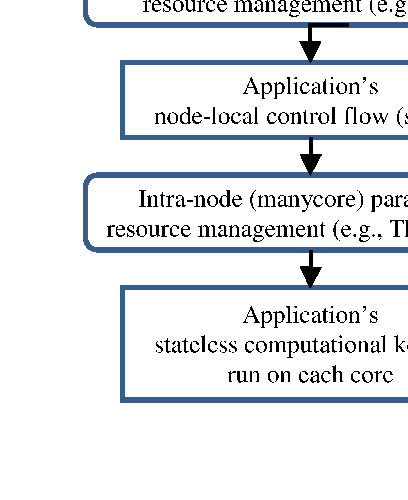
\includegraphics[viewport=0.5in 0.75in 3in 4.5in,angle=0,scale=1]{figures/HybridParallelLayers}
\caption{Software layers for the separation of concerns within HPC applications exploiting both distributed and manycore parallelism}
\label{fig:HybridParallelArchitecture}
\end{center}
\end{figure}
%
The primary objective of this layered software architecture is to separate concerns such that porting or refactoring one layer (\emph{e.g.}, manycore parallelism) has minimal impact on the remaining layers.
%
In this architecture the lowest-level computational kernels are \emph{stateless} functions that perform their computations on data provided through the manycore resource management layer.


A primary function of the intra-node (manycore) resource management layer is to dispatch the stateless computational kernels to be called in parallel on each available thread.
%
This is the intended functionality of the ThreadPool library, as well as other libraries and programming languages.
%
A well-known library supporting homogeneous manycore parallelism is the Intel Threading Building Blocks (TBB) \cite{TBB:Book}, which provides a C++ interface to manage thread-parallel execution of C++ functions.
%
A well-known language supporting heterogeneous manycore parallelism is
CUDA \cite{CUDA:WebSite},
which supports thread-parallel execution of functions written in the CUDA language on GPGPU manycores manufactured by
NVIDIA \cite{NVIDIA:Website}.


The ThreadPool library provides a simple, minimalistic, and highly portable package with which HPC applications can effectively exploit homogeneous manycore parallelism; and through which the performance implications of this architectural layer can be easily explored.
%
It is written in the standard C programming language and utilizes a small portion of the standard \textbf{pthreads} \cite{pthreads:Standard} in Linux environments.
%
This report describes the application programmer interface (API) and performance of the ThreadPool library available through the Trilinos project \cite{Trilinos:WebSite}.


